\documentclass[11pt,twoside,twocolumn,a4paper]{article}

\usepackage{acvrw}
\usepackage{times}
\usepackage{epsfig}
\usepackage{graphicx}
\usepackage{amsmath}
\usepackage{amssymb}

%%%%%%%%%%%%%%%
%% FINAL COPY %
%%%%%%%%%%%%%%%

% !!! UNCOMMENT THIS LINE FOR THE FINAL SUBMISSION !!!
% \acvrwfinalcopy 

\def\acvrwPaperID{****} % *** Enter the ACVRW Paper ID here
\def\httilde{\mbox{\tt\raisebox{-.5ex}{\symbol{126}}}}

% Pages are numbered in submission mode, and unnumbered in camera-ready
\ifacvrwfinal\pagestyle{empty}\fi
\begin{document}


%%%%%%%%%
% TITLE %
%%%%%%%%%
\title{\LaTeX\ Author Guidelines for ACVRW 2020 Proceedings}


\author{First Author, Second Author\\
Institution1\\
{\tt\small \{first,second\}@aaa.at}
% For a paper whose authors are all at the same institution,
% omit the following lines up until the closing ``}''.
% Additional authors and addresses can be added with ``\and'',
% just like the second author.
% To save space, use either the email address or home page, not both
\and
Third Author\\
Institution2\\
{\tt\small third.tauthor@xyz.org}
}


\maketitle
\ifacvrwfinal\thispagestyle{fancy}\fi

%%%%%%%%%%%%
% ABSTRACT %
%%%%%%%%%%%%

\begin{abstract}
This document gives a specification for the paper layout for submission to the 
Austrian Computer Vision and Robotics Workshop 2020. The template is based on 
the CVPR 2012 template and CVWW 2017 template. This document is written in 
accordance to the specification and guidelines, and hence may be used as an 
example of how a paper should look like.
\end{abstract}


%%%%%%%%%%%%%
% BODY TEXT %
%%%%%%%%%%%%%

%-------------------------------------------------------------------------
\section{Introduction}

Please follow the steps outlined below when submitting your manuscript to the 
ACVRW. 


\section{General information}

The reviewing process will be double-blind. The papers are expected to present 
novel work. Accepted papers will be published in the workshop proceedings via 
Verlag der TU Graz. If the paper is published in the workshop proceedings, it 
will also be available for download on our web-page (provided a single DOI). 


%-------------------------------------------------------------------------
\subsection{Language}

All manuscripts must be in English.


\subsection{Paper length} 

ACVRW papers may be of the following types:

\begin{itemize}

\item Research paper (4-6 pages)
\item Industrial or scientific spotlight (1-2 pages)
\item Student poster (2 pages)
\end{itemize}

Overlength papers will simply not be reviewed. This includes papers where the 
margins and formatting are deemed to have been significantly altered from those 
laid down by this style guide. 


%-------------------------------------------------------------------------
\subsection{The ruler}

The \LaTeX\ style defines a printed ruler which should be present in the version 
submitted for review.  The ruler is provided in order that reviewers may comment 
on particular lines in the paper without circumlocution.  The presence or 
absence of the ruler should not change the appearance of any other content on 
the page.  The camera ready copy should not contain a ruler. (Users should 
uncomment the \verb'\acvrwfinalcopy' command in the document preamble.) 


%-------------------------------------------------------------------------
\subsection{Mathematics}

Please number all of your sections and displayed equations.  It is important for 
readers to be able to refer to any particular equation.  Just because you did 
not refer to it in the text does not mean some future reader might not need to 
refer to it.  It is cumbersome to have to use circumlocutions like ``the 
equation second from the top of page 3 column 1'' (Note that the ruler will not 
be present in the final copy, so is not an alternative to equation numbers). 


%-------------------------------------------------------------------------
\subsection{Color}

Color is valuable, and will be visible to readers of the electronic copy. 
However ensure that, when printed on a monochrome printer, no important 
information is lost by the conversion to grayscale. 


%-------------------------------------------------------------------------
\subsection{Citations, Tables, and Figures}

One could cite works on Frobnication \cite{Alpher02, Alpher03}, or work of 
Alpher~\etal~\cite{Alpher04}. Tables and figures help the reader to better 
understand the content. For instance, Figure~\ref{fig:onecol} shows the floor 
plan of of the mathematics building of TU Graz, where the workshop will take 
place. In addition, Table~\ref{tab:participants} gives an overview on the 
co-located workshops of OAGM and ARW:  

\begin{table}
   \centering
   \begin{tabular}{|l|c|}
   \hline
    Location & Year \\
   \hline\hline
   Wels, Austria  & 2016 \\
   Vienna, Austria  & 2017 \\
   Steyr, Austria  & 2019 \\
   Graz, Austria  & 2020 \\
   \hline
   \end{tabular}
   \caption{Co-located OAGM and ARW workshops.}
   \label{tab:participants}
\end{table}


\begin{figure}
   \centering
   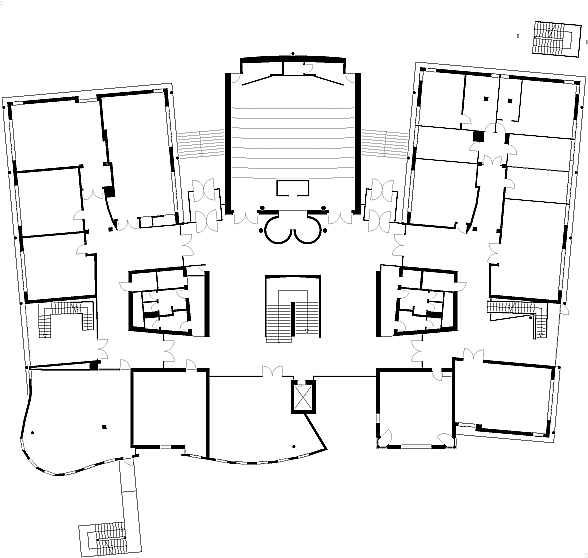
\includegraphics[width=0.65\columnwidth]{STEG.png}
   \caption{Floor map for ACVRW 2020.}
   \label{fig:onecol}
\end{figure}


%-------------------------------------------------------------------------
\section{Conclusion}

Please do not forget to replace the asterisks in the example paper with your 
paper's own ID before uploading your file. You receive a paper ID by generating 
a new submission without adding a file. Submissions can be edited until the 
deadline. 


%-------------------------------------------------------------------------
\section*{Acknowledgments}

Are acknowledgments OK?  Yes, but leave them for the final copy.


{\small
\bibliographystyle{ieee}
\bibliography{acvrw}
}

\end{document}
